\documentclass{article}
\usepackage[utf8]{inputenc}
\usepackage{graphicx}
\usepackage{fullpage} % Makes full page size


\title{Epigenetic simulation manuscript}
\author{Holly V. Moeller and the E5 Rules of Life Team }
\date{}

\begin{document}

\maketitle

\section{NOTES TO COAUTHORS: Paper framework}


\noindent \textbf{TARGET JOURNAL: Ecology Letters ``review and synthesis''}   

The goal of this paper is to use a simple epigenetic simulation as a framework to (1) synthesize the current state of understanding about the role of epigenetics in environmental matching, and (2) identify open questions in epigenetics research that should be prioritized. 

One way in which the paper could be organized would be by including a series of sections, each of which presents a core model prediction. Following presentation of the model's prediction, the section could review empirical evidence and then identify open avenues of research.

The outline/structure below follows this approach.

For now, I have left the Introduction blank, and put in placeholders for ``empirical data'' and ``knowledge gap'' in each section. (For each of these, there is some italicized text with a few ideas I had that maybe could be fleshed out.)

I could use your help with:
\begin{itemize}
    \item Providing feedback on bold-faced queries/thoughts in the text.
    \item Identifying key topics or themes that could fit into the ``empirical data'' and ``knowledge gap'' sections for each part of the paper.
    \item Actually writing some of that text!
    \item Brainstorming about how to frame this paper (and conclude it) in a way that would appeal to a broad audience at, e.g., \textit{Ecology Letters}.
\end{itemize}

\section{Introduction}

TKTKTK

\section{The Model}
Here we present a simple simulation model that is intended to represent the iterative process of adding and removing epigenetic markers to an organism's genome. For simplicity, we can think of these markers as methyl groups that are attached to cytosines. 

An organism's methylation pattern influences its gene expression. Depending upon environmental conditions, certain gene expression strategies may be more favorable than others; an organism that adjusts its epigenetic state accordingly will therefore be better matched to its environment. Thus, organisms that are poorly matched to their environment should experience physiological benefits if they change their epigenetic markers to improve their match to the environment.

Here, we mimic this phenomenon by assuming that an organism experiences ``stress'' that is proportional to its mismatch with local environmental conditions. The more stress an organism experiences, the greater the rate at which it remodels its epigenetic state. In some incarnations of the model, increased stress can also influence birth-death processes if we assume that the organisms with the highest stress levels are most likely to die, and the ones with the lowest stress levels are most likely to reproduce.

\subsection{Model Components}

\textbf{HVM to revise this text carefully to use 1 as presence and 0 as absence of epigenetic markers. Generally mechanism-agnostic; empiricists will add examples for multiple mechanisms where the directionality (e.g., methylation means gene expression or prevention) varies. Also back away from markers as methylation. I.e. $1 = $ presence of epigenetic marker (not methylation).}

\ 

\noindent \textit{The Environment}: We represent the environment as a binary string of 1s and 0s, $\vec{E}$. Each of the $n$ positions in the string represents a hypothetical location in an organism's genome that could take on one of two epigenetic states in response to environmental conditions. The environmental string's value at a particular position $E_i$ (which is either 1 or 0) represents the organismal epigenetic state that would be best matched to the environment. There are many possible interpretations of a single position on this string, which could represent a specific cytosine which should be methylated (=1) or demethylated (=0), or a gene or suite of genes corresponding to a particular phenotype that should be expressed (=1) or not expressed (=0) in order to best match the environment. (It's best to think of this binary string as corresponding to the suite of an organism's genes that can be environmentally responsive. That is, we are neglecting genes that are silent or constitutively expressed, or that have invariant epigenetic states.)

The environment can vary. There are many ways of implementing environmental change (i.e., shifts of $E_i$ from $0$ to $1$ or vice versa). We consider two possibilities: In one case, we periodically re-draw the entire environmental string, which represents an ``extreme event'' with an abrupt and random perturbation. In the second case, we allow the environment to vary cyclically by gradually shifting the environmental epigenetic state over time in a systematic manner. In this case, we can control both the speed (frequency of shifts) and magnitude (number of changed epigenetic sites) of environmental change, allowing us to mimic perturbations like seasonality, interannual variation, and decadal cycles.
%(Other possibilities include: partial re-drawing, or a cyclic change representing seasonality.) Generally, environmental change is rare  compared to organismal epigenetic change, although environmental changes are large in magnitude when they occur (representing ``extreme events'').
\ 

\ 

\noindent \textit{The Organisms:} We use an individual based model to represent the population of living organisms in our model. Each individual is represented by its own binary string, $\vec{O}_j$, of the same length as the environmental string. Each position on an organism's string corresponds to the same position in the environmental string; this allows an individual organism to experience variable degrees of ``stress'' depending on the number of sites that are mismatched with the environment. Organisms can modify their epigenetic state according to the mechanisms outlined below, and may experience birth-death processes (with or without mutational change), depending upon the model formulation that is used. Again, there are various interpretations of an ``organism'' in this model. For example, we could also think of each string as representing the nuclear genome of a single cell in a multicellular organism, or as representing the median state of an entire organism. \textbf{(NOTE: The assumption of a binary (either 0 or 1) state might lend itself more to the interpretation of a single cell.)}

\ 

\noindent \textit{Stress-Dependent Epigenetic Change:} We can quantify the amount of stress an organism is experiencing based on its average degree of mismatch with the environment across all $n$ possible epigenetic sites. Individual $j$'s level of stress $S_j$ is therefore given by:
\begin{equation}
   S_j = \frac{\sum_i ^n | E_i - O_{j,i} |}{n} .
\end{equation}
Note that this approach assigns each epigenetic location equal weighting, and assumes that incorrectly methylated sites (i.e., organism = 1, environment = 0) and incorrectly demethylated sites (i.e., organism = 0, environment = 1) are equivalently stressful.

We assume that an organism makes epigenetic modifications proportional to the level of stress it is experiencing. In other words, if an organism is well-matched to its environment, its stress levels are low, and it will make few, if any, epigenetic changes. But when an organism's stress levels are high, it will accelerate rates of epigenetic remodeling in an attempt to more quickly achieve environmental optimality. Therefore, we represent each organism's probability of adding an epigenetic marker to a single site (i.e., changing that site's epigenetc state from a 0 to a 1, such as via methylation) within a round of epigenetic modification as proportional to its current stress level $S_j$, scaled by an individual-specific methylation tendency $m_j$:
\begin{equation}
    M(j,t) = \min\left[m_jS_j(t),1\right].
\end{equation}
This stress-dependent probability is used to determine whether or not a currently demethylated site is methylated during a given round of epigenetic change. Specifically, for each demethylated site, the algorithm draws a value between 0 and 1 from a uniform distribution. If this value is greater than the methylation probability $M(j,t)$, the site is methylated. Per-round probabilities are capped at 1. Statistically, this means that the total number of sites that are methylated in a given is drawn from a binomial distribution with a probability $M(j,t)$ and a number of trials equal to the number of presently demethylated sites (state = 0). 


Demethylation is scaled similarly, with an individual demethylation tendency $d_j$:
\begin{equation}
    D(j,t) = \min \left[d_jS_j(t),1 \right].
\end{equation}

Methylation and demethylation probabilities tell us how likely an organism is to remodel each position in its string $\vec{O}_j$ at each timestep. However, these probabilities may change if the organism has information about which sites are currently mis-matched with its environment. Such environmental information might be collected when, for example, gene products inhibit gene expression. When environmental conditions halt the use of these gene products, the gene is then occluded, and epigenetic markers can be removed. \textbf{(-- NB: Need help here to think of a good example for why feedback is in demethylation!)} We use a scalar to increase the probability of ``correct'' epigenetic changes. Thus, the probability of demethylating a mismatched site (i.e., location where the environmental state is 0 and the organismal state is 1) is given by:
\begin{equation}
    D_p(j,t) = \min\left[(p_j+d_j)S_j(t),1\right].
\end{equation}
where $p_j$ is the individual-specific preferential demethylation tendency. Although both methylation and demethylation can occur preferentially, here we consider only preferential demethylation. \textbf{(NB: Made this choice to get ``spikes'' in demethylation after an environmental change. Maybe consider the alternate case in a supplement?)}

Because similar cellular equipment is likely used for both preferential and baseline removal of epigenetic markers, we assume that these two probabilities must be related to one another. In other words, if an organism has produced a lot of cellular enzymes that demethylate cytosines, then these enzymes may increase both informed (e.g., $p_j$) and random (e.g., $d_j$) demethylation tendencies. We therefore assume that there is an overall demethylation tendency $o_j$, that is governed by the production of such machinery, and that an environmental information parameter, $\epsilon$, links the random and preferential change tendencies, which are centered around this overall tendency:
\begin{equation}
    o_j = \frac{ d_j\left( 1 - \epsilon \right) + p_j \left( 1+ \epsilon \right) }{2}.
\end{equation}
Here, we choose $0 \leq \epsilon \leq 1$ so that all demethylation probabilities are nonnegative.

It is convenient to link the addition and removal of epigenetic markers, which we do with the parameter $b$, that scales the tendency of removal relative to the tendency of addition:
\begin{equation}
    m_j = b o_j = \frac{b\left[ d_j\left( 1 - \epsilon \right) + p_j \left( 1+ \epsilon \right) \right]}{2}.
\end{equation}
If $b > 1$, demethylation is more stress-sensitive than methylation, and if $b < 1$, the opposite is true.

In our simulations, we focus on an environment that has roughly equal numbers of methylated and demethylated sites. That is, the proportion of epigenetic sites that is in state $1$ is approximately $0.5$. Thus, an organism whose genome is wholly methylated and an organism whose genome is wholly demethylated both experience high stress levels of $0.5$, which is also the mean expected stress level of an organism with an entirely random epigenetic strategy. \textbf{(This paragraph kind of feels like it belongs in the ``environment'' description, but I needed to define stress first, which only shows up in the organism section...)}

\ 

\noindent \textit{Birth-death processes:} Occasionally (that is, less frequently than epigenetic remodeling; see section on timescales below), organisms experience mortality. We assume that natural selection acts on the population, such that when a birth-death event occurs, organisms that are presently experiencing the highest levels of stress are the most likely to die. Meanwhile, organisms with the lowest stress levels are most likely to reproduce. Our current algorithm assumes strong natural selection, such that the organism with the highest stress is eliminated (= death event), and the organism with the lowest stress is duplicated (= birth event). Birth events duplicate an organism's parameters (e.g., $m_j$ and $d_j$) as well as its present epigenetic state $\vec{O}_j$.

\ 

\noindent \textit{Mutation:} Mutational events can impact an organism's tendency for methylation or demethylation. When a mutation event happens (which is even less frequent than a birth-death event), we draw a new tendency from a normal distribution centered around the organism's present tendency. Tendencies are constrained to be non-negative; thus a mutation that results in $m_j<0$ or $d_j<0$ will be rounded to $m_j=0$ or $d_j=0$, respectively.


\subsection{Algorithm Steps}
In our model, at each time step, events occur in the following order, for each individual:
\begin{enumerate}
    \item The individual's stress is computed.
    \item Methylation (changes from 0 to 1) occurs.
    %\item Stress is re-computed. \textbf{NOTE: Results don't really change if I skip this step, or if I swap order of methylation and demethylation. Let's talk about what choices are best?}
    \item Demethylation (changes from 1 to 0) occurs.
\end{enumerate}

Following these individual events, population-level events occur in the following order. Note that not all events take place at every time step:
\begin{enumerate}
  \setcounter{enumi}{4}
    \item A single birth-death event, if any, occurs.
    \item A single mutation event, if any, occurs.
    \item Environmental change, if any, occurs.
\end{enumerate}

\textit{A note on timescales:} In our model, events occur with different frequencies. In order from most frequent to last, we have:
\begin{enumerate}
    \item Epigenetic changes. These occur every timestep, although the rate at which they occur depends upon an organism's propensity for methylation and demethylation.

    \item Mutational change and birth-death processes. These occur less frequently than epigenetic changes, but more frequently than environmental shifts. We generally assume that birth-death events are more frequent than mutations, so that the fitness effects of a mutation can play out for several generations.

    \item Environmental change. Shifts in the environment are relatively rare, and occur about once every 100 epigenetic timesteps. 
\end{enumerate}

The frequency of each of these events implies an interpretation of the model's timescale. For example, the frequency of epigenetic change with respect to generation time implies that we are modeling within-generation epigenetic change, rather than epigenetic remodeling that occurs only during reproduction.


\begin{figure}
    \centering
    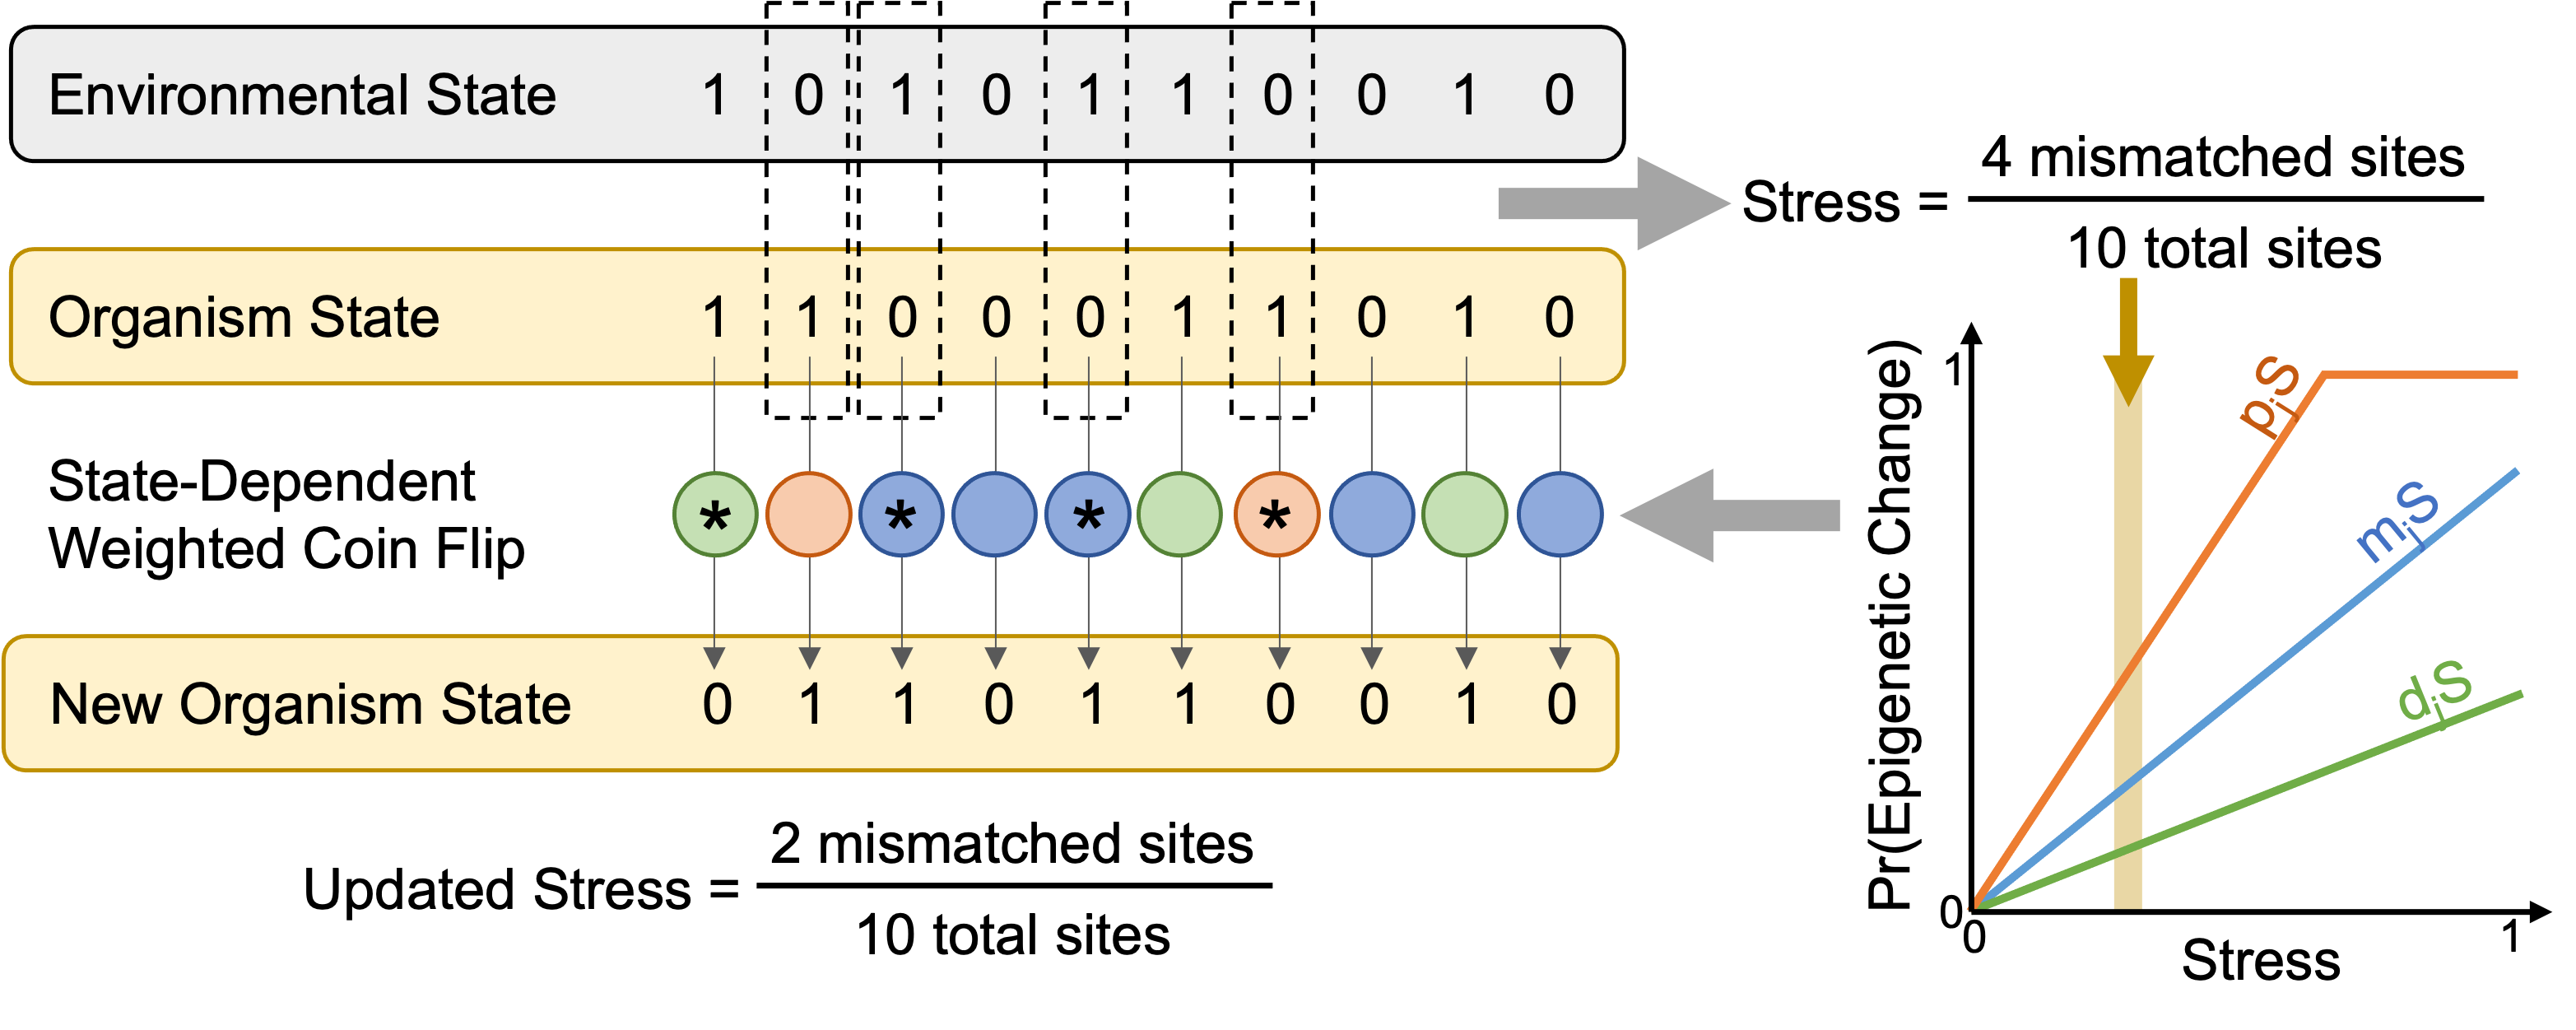
\includegraphics[width=\textwidth]{Figures/ModelDiag_v1.png}
    \caption{Conceptual diagram showing epigenetic modification. First, the organism's state is compared to the environment and stress is computed. Based on stress levels and epigenetic change tendencies, the probability of an epigenetic change is computed. These probabilities are used to weight ``coin flips'' that determine which specific locations in the genome undergo methylation (blue), demethylation (green), or preferential demethylation (orange). In the diagram, coin flips that result in epigenetic change are marked with a star. Following these changes, the organism's stress can be recomputed (beginning the next timestep); in this case, stress has been reduced from 0.4 (4 mismatched sites) to 0.2.}
    \label{fig:modeldiag}
\end{figure}

\subsection{Model Analysis}
We used our model to address three questions about how epigenetic modifications could allow organisms to track their environment. We asked (1) whether organisms must receive some information about the state of the external environment in order to be able to track the environment; (2) what relative rates of addition and removal of epigenetic markers allow an organism to minimize its stress by tracking its environment; and (3) under which environmental conditions epigenetic change is an effective mechanism for environmental tracking. Below, we describe our analytical approach and the model's predictions for each query. We compare the model's predictions with existing empirical knowledge, and identify key research priorities to address any knowledge gaps.





\clearpage

\section{Results}

\subsection{Tracking the environment requires information}
How do organisms gather information about the environment around them, and is this information necessary for them to tune their epigenetic state to match environmental needs? While stress from environmental mismatch can be measured at the aggregate scale, it is less clear how organisms might identify which specific genes should be activated or deactivated based on environmental cues. Therefore, we first used our model to investigate what information organisms need to detect about their (mis)match to the environment in order to track the environment epigenetically.

\subsubsection{Model Results}
We contrasted the ability of an organism to track a stochastically changing environment as a function of its degree of information about the state of that environment. Specifically, we varied the magnitude of the difference between preferential and random demethylation probabilities as a proxy for the amount of information an organism has about its environment. When epigenetic state is driven entirely by feedbacks cementing the expression of necessary gene products, then the only sites chosen for demethylation are those that produce matches to the environment. In this case, $\epsilon = 1$, such that $d_j = 0$ and $p_j = 2m_j$. 


We found that, in the absence of birth-death processes that vertically transmit preferable epigenetic states via natural selection, only organisms that can obtain environmental information are able to track the environment (Figure \ref{fig:envfeedback}). Populations of these organisms experience transient increases in stress when the environment changes correlated with periods of demethylation (Figure \ref{fig:envfeedback}b). Over time following the environmental perturbation, these organisms adjust their epigenetic state to match their environment, lowering their stress levels from $\approx 0.5$ (the mean expected proportion of mismatched sites when the environment and organism are drawn randomly) to lower values over time. 

The magnitude of stress reduction depends on how successfully the organism can decouple random ($d_j$) and preferential ($p_j$) demethylation (Figure \ref{fig:envfeedback}c). The optimal solution would be to set $d_j = 0$ so that no random demethylation occurs, and increase $p_j$ without bound so that the probability of accurately demethylating mismatched sites is high, even when stress is low. However, it seems unlikely that an organism would be able to completely avoid inadvertent demethylation, especially when there is high expression of enzymes related to this process in response to stress (i.e., if $p_j$ is large). Thus, in our subsequent analyses, we coupled these rates to each other by setting $\epsilon = 0.8$. \textbf{I chose 0.8 for interesting dynamics, but probably need to talk about this w/ the empiricists.}


\begin{figure}
    \centering
    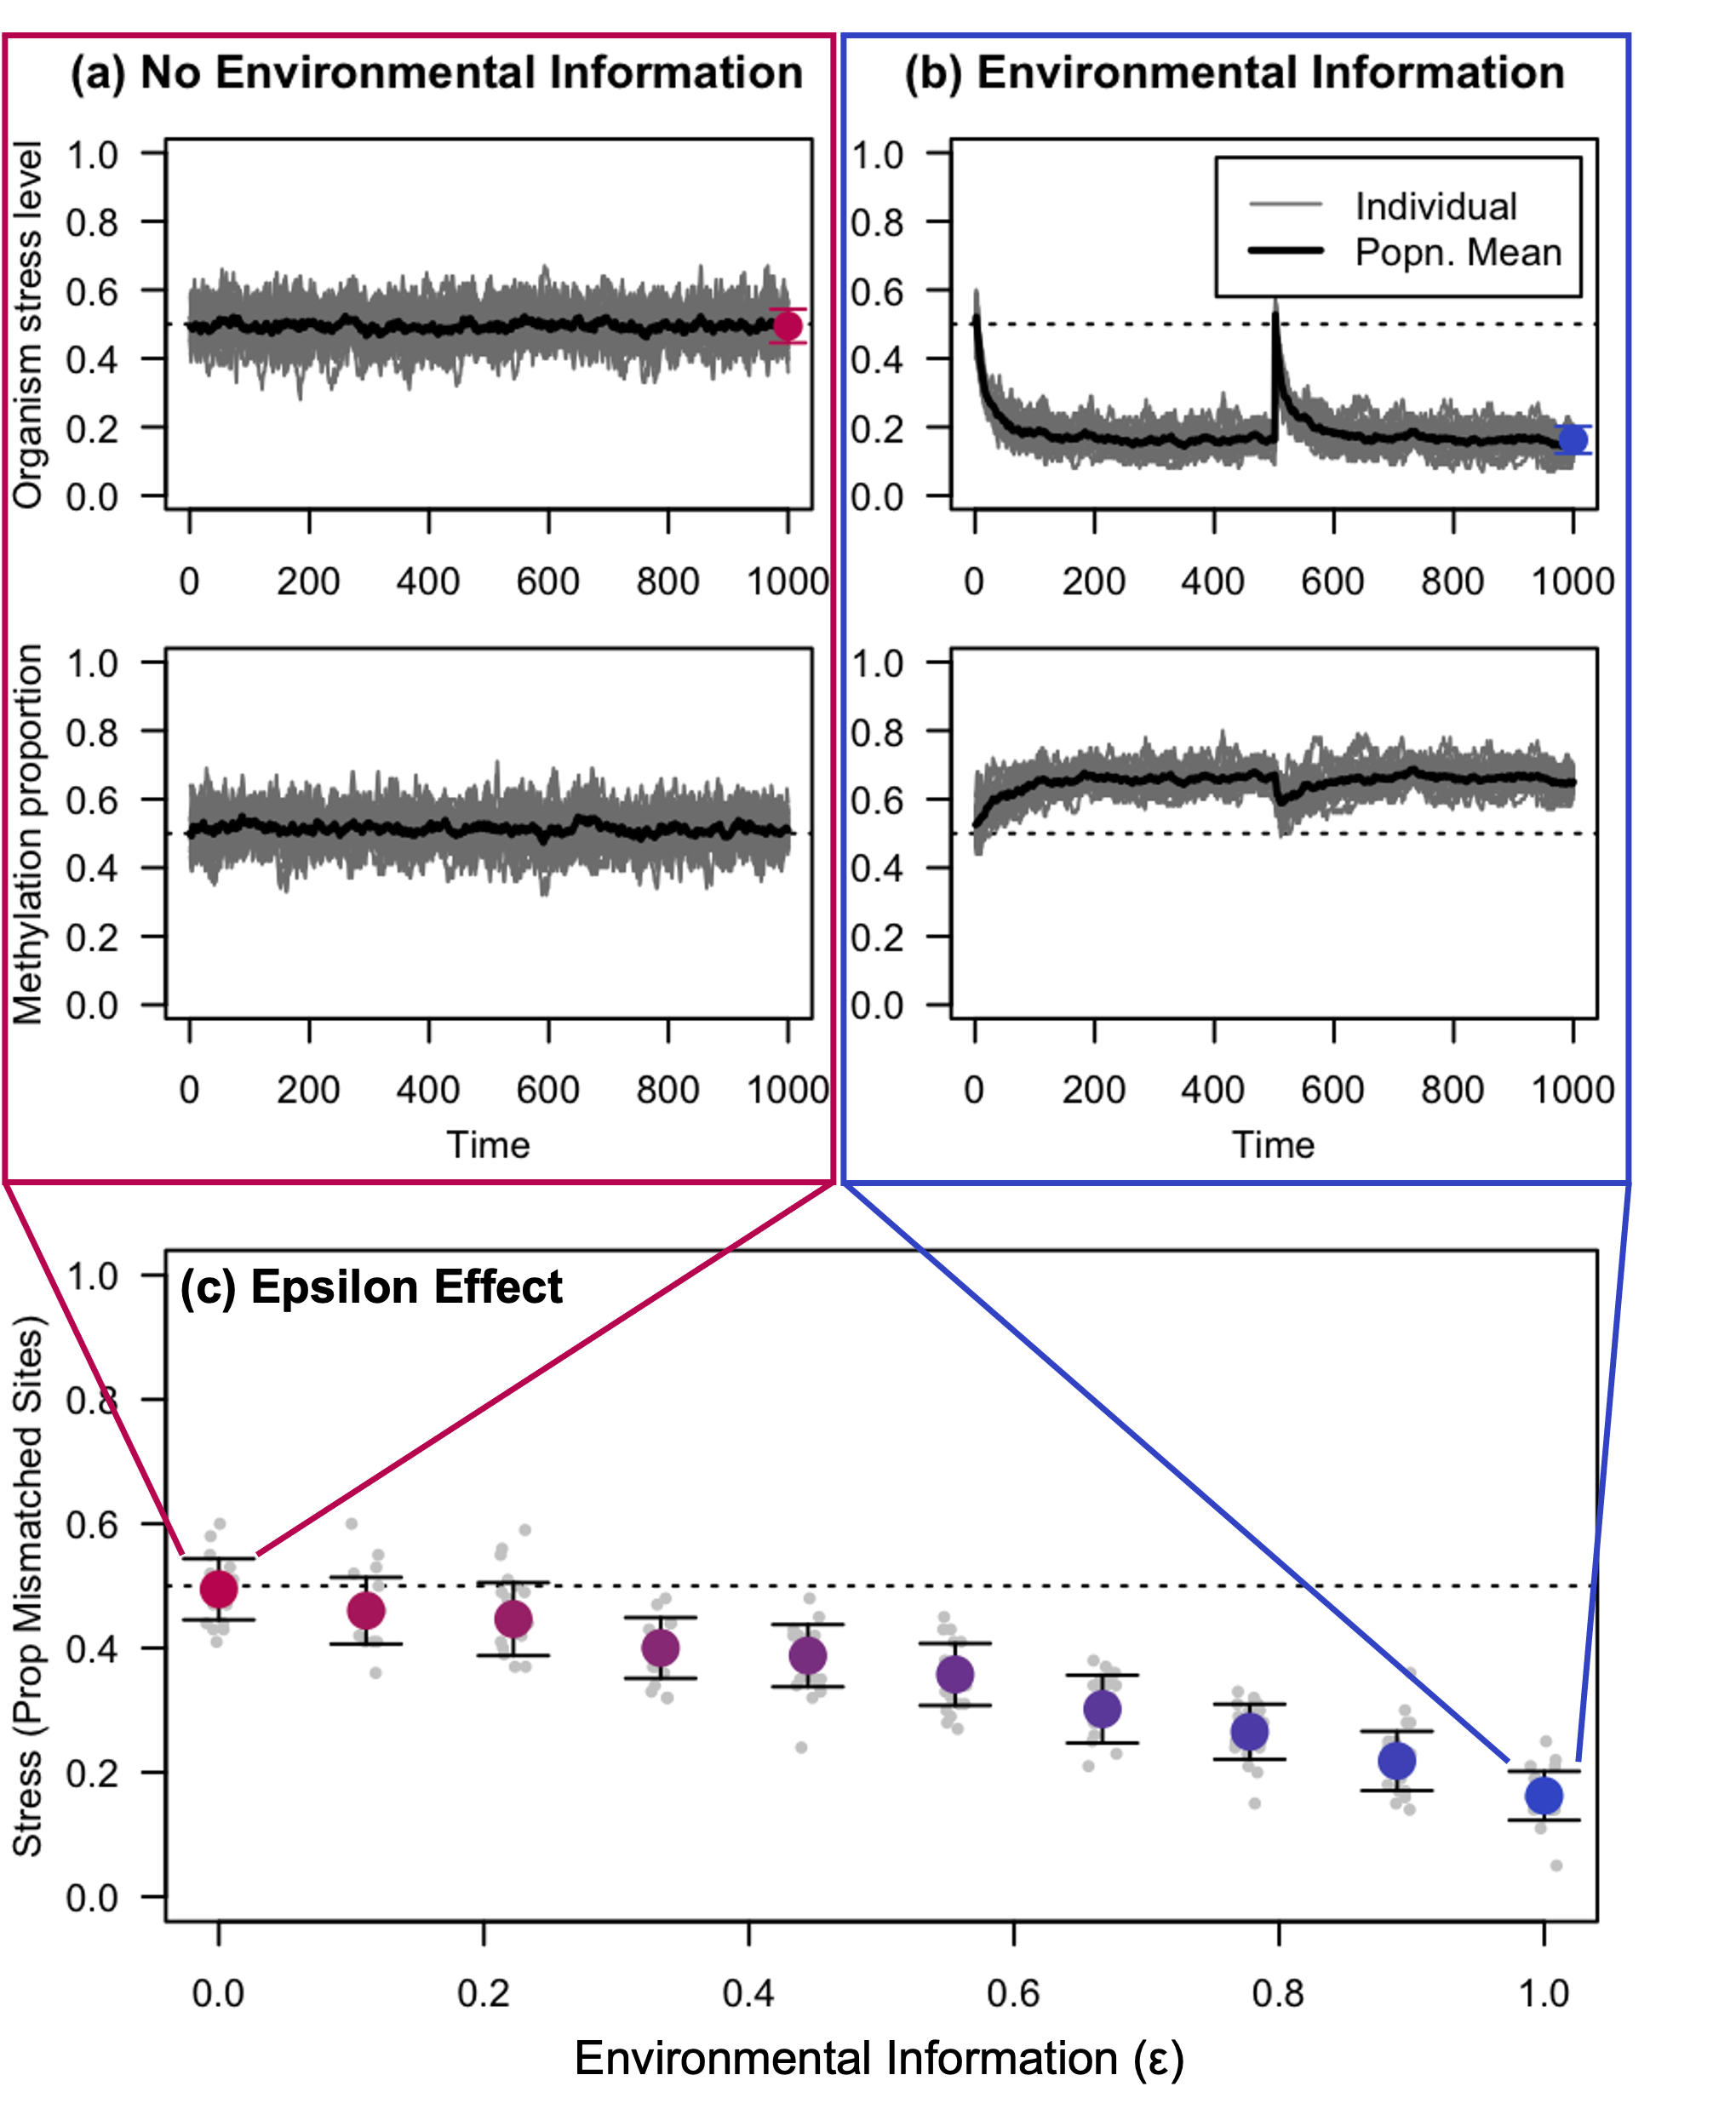
\includegraphics[width=.8\textwidth]{Figures/Fig_EnvironmentalFeedback_Consolidated.png}
    \caption{\textbf{Effects of environmental information on organismal stress.} Top: Timeseries showing a group of 20 organisms tracking (or failing to track) their environment over time. Without environmental information stress levels hover around the mean expectation of 0.5 (a), but with environmental information, the organisms are able to reduce their stress levels within about 100 timepoints (b). Bottom: The larger the difference in baseline and preferential demethylation tendencies, the better the organism's performance. Simulations are for 50 organisms with a baseline methylation tendency of 0.2. Bars show standard deviation around the mean.}
    \label{fig:envfeedback}
\end{figure}


\subsubsection{Empirical Data}

\textit{Data showing that organisms remodel their epigenetic state following a perturbation, especially if that involves transient demethylation}

\ 

\textit{Evidence for mechanisms that can transmit ``environmental information'' and allow an organism to target how it adds/removes epigenetic markers.}


\subsubsection{Knowledge Gap}

\textit{Exact mechanisms of how epigenetic targetting is done, how organisms upregulate or downregulate machinery to make epigenetic modifications, etc.}



\clearpage

\subsection{``Optimal'' coupling of epigenetic change tendencies depends on the environment}

The dynamic process of adding and removing epigenetic markers allows for the location of these markers to shift over time, enabling an organism to respond to changes in its environment. However, in order to maintain epigenetic states, the loss and addition of these markers must be roughly balanced. Therefore, we next studied how methylation and demethylation tendencies (which in our model underlie the linkage between an organism's stress and its rate of epigenetic change) must be coupled to one another in order to allow for epigenetic tracking.


\subsubsection{Model Results}

If methylation and demethylation probabilities become too decoupled, an organism can become completely demethylated (if $b >> 1$ such that $d_j, p_j >> m_j$) or completely methylated (if $b<<1$ such that $m_j >> d_j,p_j$). In an environment with an average methylation of $0.5$ (as studied here), an organism that has lost (or gained) all of its epigenetic markers experiences a high level of stress (0.5), so the more mismatched the probabilities, the higher the stress level (Figure \ref{fig:methylmismatch}).

\begin{figure}
    \centering
    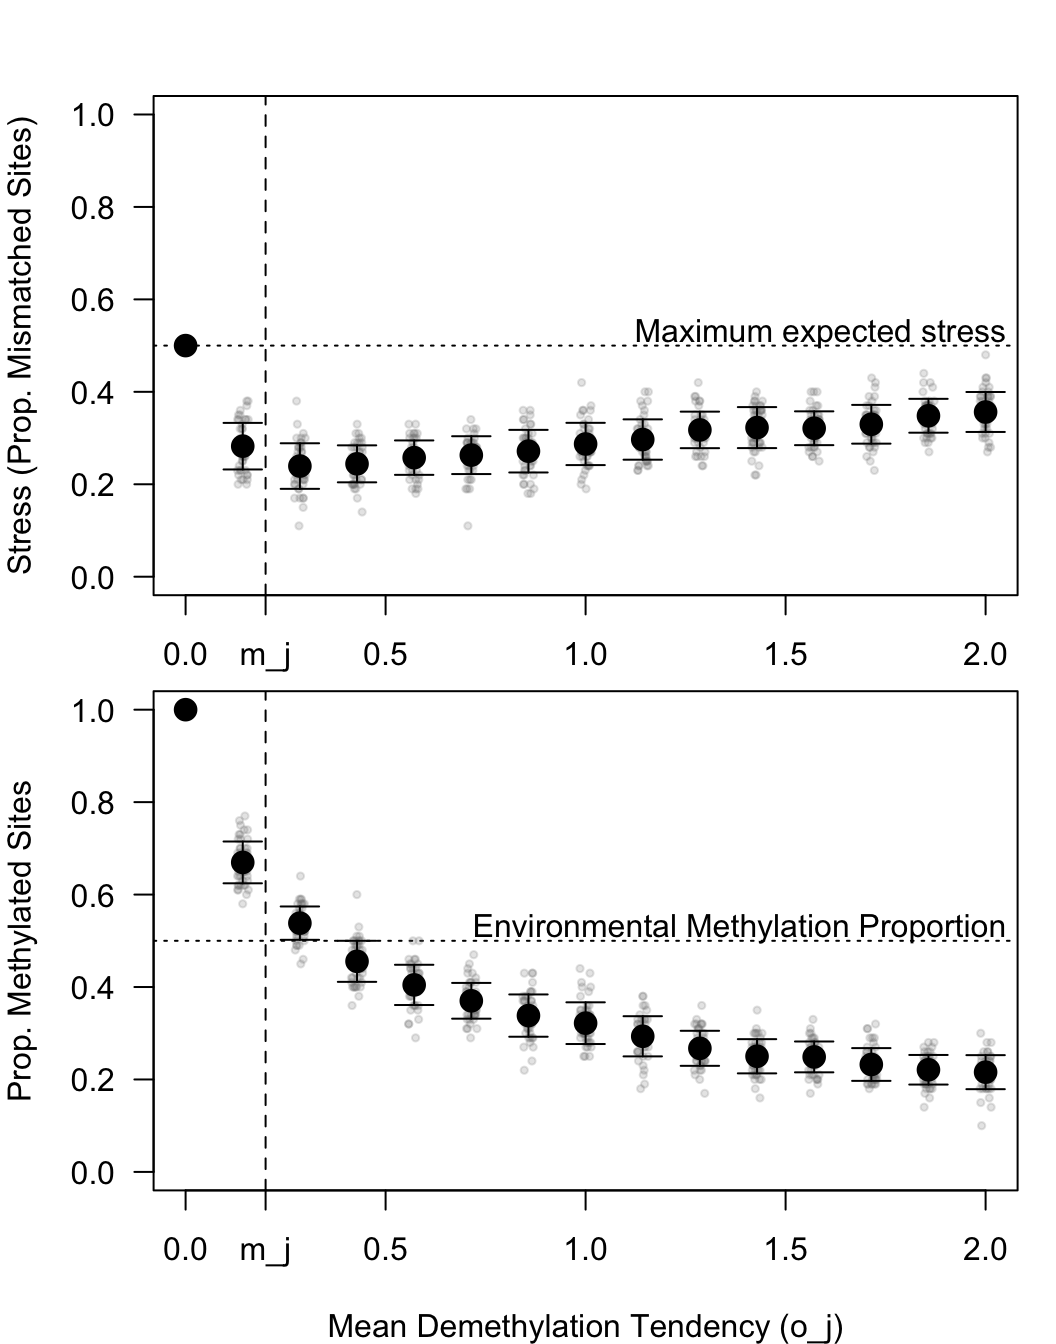
\includegraphics[width=0.8 \textwidth]{Figures/Fig_DemethDependence.png}
    \caption{\textbf{FOR SUPPLEMENT:} Dependence of stress and proportion sites methylated on demethylation tendency. Stress is minimized when mean demethylation tendency ($o_j$) is similar to methylation tendency ($m_j$) and the proportion of methylated base pairs is similar to but slightly higher than the environment (0.5). Simulations are for 50 organisms with a baseline methylation tendency of 0.2 (vertical dashed line). Bars show standard deviation around the mean. The null expectation for stress and the proportion of environmental sites methylated (0.5, dotted horizontal line) are also shown for reference. }
    \label{fig:methylmismatch}
\end{figure}

We computed optimal pairs of methylation and demethylation tendencies by fixing the former and using a pseudo-evolutionary algorithm to find values of the former that minimized organismal stress. Specifically, we modified our algorithm to include birth-death processes that eliminated the highest stress individual and replaced that individual with a duplicate of the lowest stress individual (mimicking reproduction of the highest fitness individual). Birth-death processes occurred every 10 rounds of epigenetic change, and every tenth birth-death event also involved a mutation in the demethylation tendency. When a mutation occurred, a new mean demethylation tendency was drawn from a normal distribution with standard deviation 0.1 centered around the parent's demethylation tendency. We bounded the distribution at zero, so that negative tendencies could not arise. Thus, over time, populations evolved demethylation tendencies that minimized stress (Figure \ref{Sfig:evolutionts}). %We repeated this pseudo-evolutionary approach for several rounds to confirm our findings.

Our results highlight the importance of coupling between methylation and demethylation tendencies. Generally, higher methylation tendencies necessitate higher demethylation tendencies so that the average level of genome methylation remains constant (Figure \ref{Fig:Evolution3panel}). Decoupling between these rates produces high stress either because of rampant demethylation (if $o_j > m_j$) or methylation (if $o_j < m_j$) (Figure \ref{SFig:StressHeatmap}). However, the exact coupling of these tendencies depends upon environmental conditions. For example, when the environment has relatively few epigenetic markers, demethylation should outstrip methylation to keep the organism's overall methylation levels low (Figure \ref{Fig:Evolution3panel}a), but high environmental methylation necessitates relatively low demethylation tendencies (Figure \ref{Fig:Evolution3panel}).


\begin{figure}
    \centering
    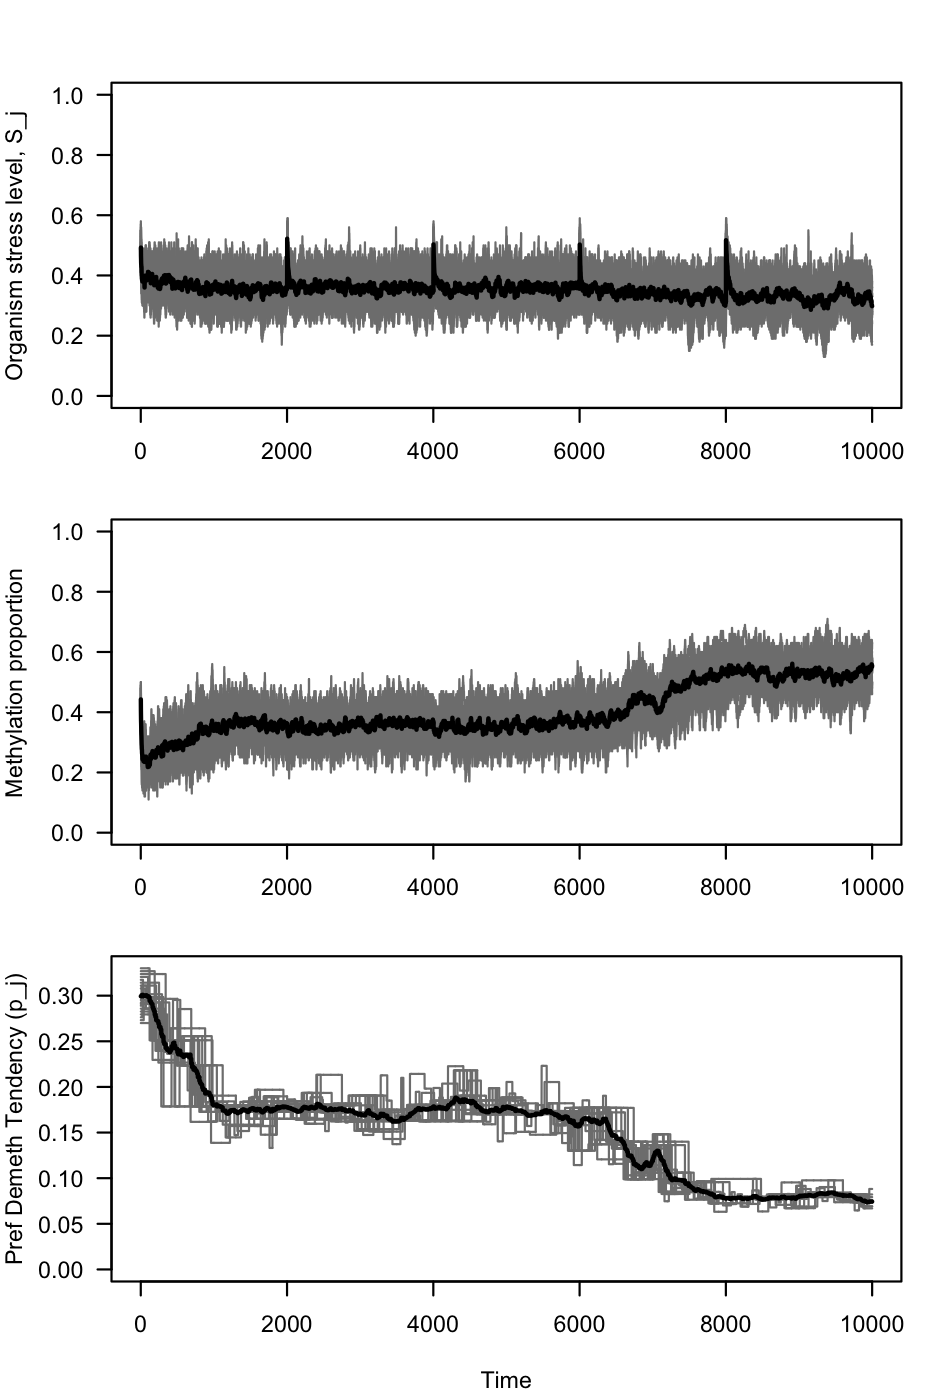
\includegraphics[width=0.8 \textwidth]{Figures/SFig_EvolutionSims.png}
    \caption{\textbf{FOR SUPPLEMENT:} Evolutionary trajectory of a population with a decreasing demethylation tendency over time. The population is subjected to periodic environmental perturbations, which it recovers from, with decreasing stress as beneficial mutations accumulate. These mutations act to reduce the demethylation tendency and thus increase the overall genomic level of methylation to closer to the environmental mean of 0.5.}
    \label{Sfig:evolutionts}
\end{figure}


\begin{figure}
    \centering
    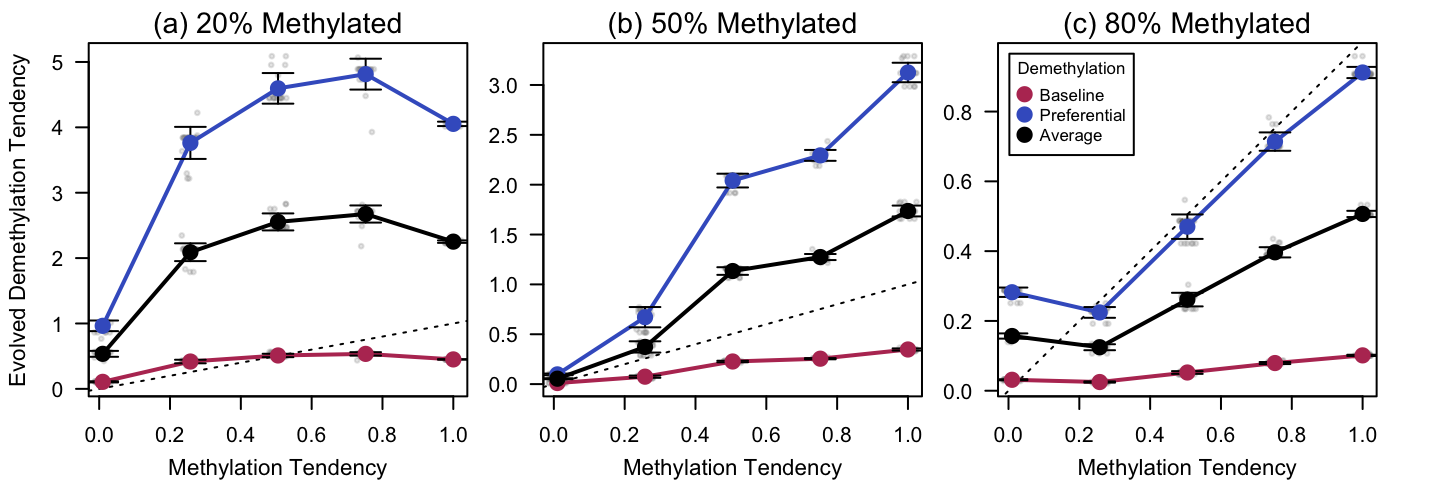
\includegraphics[width= \textwidth]{Figures/Fig_EvolutionSimulation_3cases.png}
    \caption{Evolved stress-minimizing demethylation tendencies as a function of (fixed) methylation tendencies. Note that baseline and preferential demethylation are coupled by $\epsilon = 0.8$. Generally, as an organism's tendency to methylate in response to stress increases, its tendency to demethylate increases proportionately. The more methylated the environment that the organism is tracking, the lower the evolved demethylation rates (compare from left to right, noting differences in y-axis scales).}
    \label{Fig:Evolution3panel}
\end{figure}

\begin{figure}
    \centering
    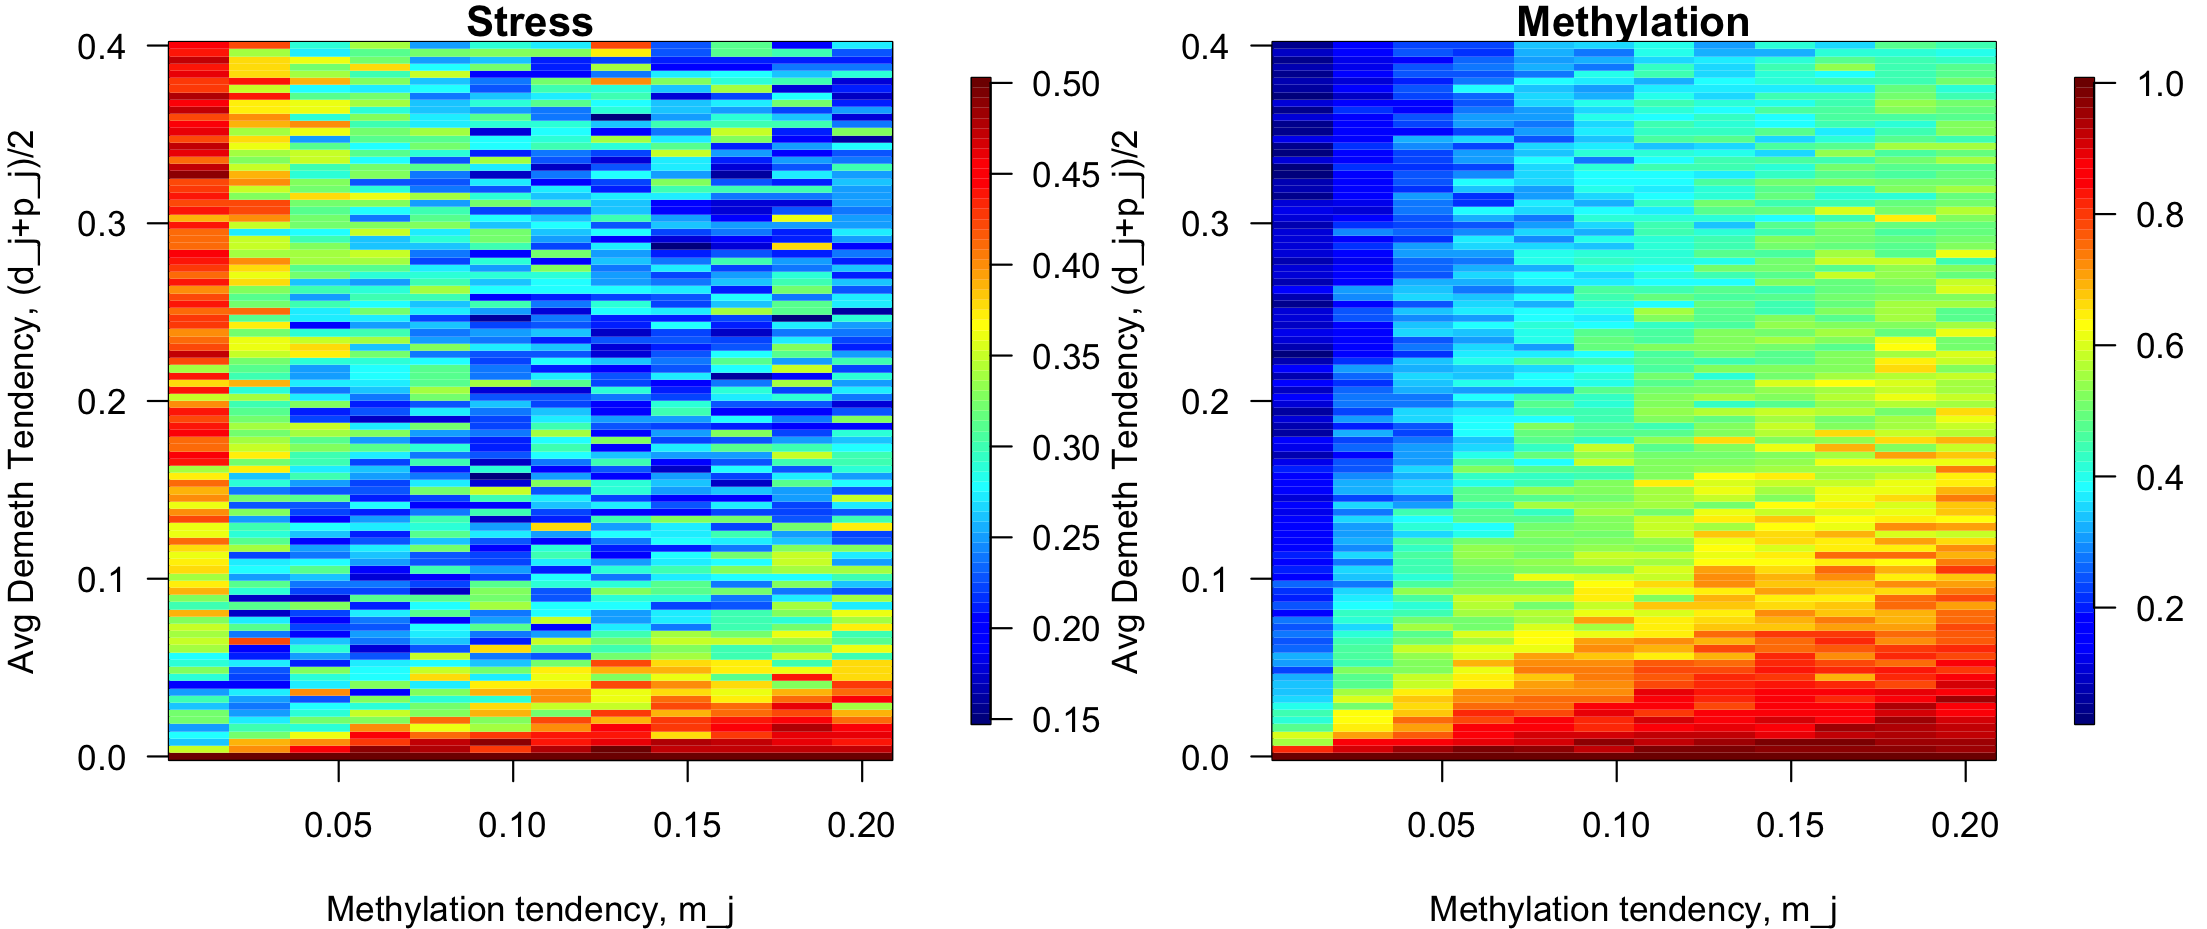
\includegraphics[width= \textwidth]{Figures/Fig_Heatmap_v2.png}
    \caption{\textbf{FOR SUPPLEMENT:} Effects of mismatched epigenetic tendencies on organism performance. If demethylation tendencies are much higher than methylation tendencies (upper left of both panels), stress is high (left panel) because the organism's methylation state is low compared to the environment (right panel). In contrast, relatively low demethylation tendencies lead to high methylation and also high stress (lower right of panels).  }
    \label{SFig:StressHeatmap}
\end{figure}


\subsubsection{Empirical Data}

\textit{Data on maintaining constancy of epigenetic state over time, data on production of machinery that adds and removes epigenetic markers?}

\subsubsection{Knowledge Gap}

\textit{Understanding how these rates are actually coupled in practice?}




\clearpage

\subsection{Tracking is only effective in certain environments}

Although epigenetic modifications can, in principle, allow organisms to become locally adapted to their environment, epigenetic change must occur on a similar timescale to environmental change to be effective.


\subsubsection{Model Results}

We used our model to explore the relationship between the frequency and magnitude of environmental change and organism stress. To do this, we first implemented a new algorithm for environmental change that allowed the environment to change with predictable fluctuations. Specifically, we simulated a ``band'' of optimally methylated environmental sites that shifted in genome location with a fixed frequency (per number of simulation timesteps) and magnitude (number of genome sites). Examples of how this model can be tuned from periodic, large changes to more frequent, small changes can be seen in Figure \ref{fig:envirovar}.

When environments change relatively rarely (e.g., once every 200 timesteps; Scenario 1 in Figure \ref{fig:envirovar}), organisms with high-information tracking strategies are able to shift their epigenetic state alongside environmental change, minimizing stress even if the environmental change is large in magnitude. However, frequent environmental changes can only be tracked if they are small in magnitude (e.g., Scenario 2 and upper right corner of Figure \ref{fig:envirovar}), and otherwise produce high levels of stress that are comparable to a random epigenetic strategy (expected mean stress of $0.5$).

Our model does not consider any costs for epigenetic modifications, so an organism that attempts to track its environment cannot incur any fitness costs in excess of its mismatch. Thus, our model cannot be used to demonstrate tradeoffs between epigenetic tracking and energy conservation, and does not have selection pressure to reduce epigenetic modification. Incorporating such costs would, however, reveal ``optimal'' epigenetic modification strategies, including abandoning epigenetic change when environmental tracking benefits are less than energetic costs.

\subsubsection{Empirical Data}

\textit{Data on variation in usage of epigenetics across different lineages, especially relating to the types of environments they come from?}

\subsubsection{Knowledge Gap}

\textit{Comparative studies of organisms in low vs high fluctuating environments, to ask which ones have epigenetic tracking modifications?}

\begin{figure}
    \centering
    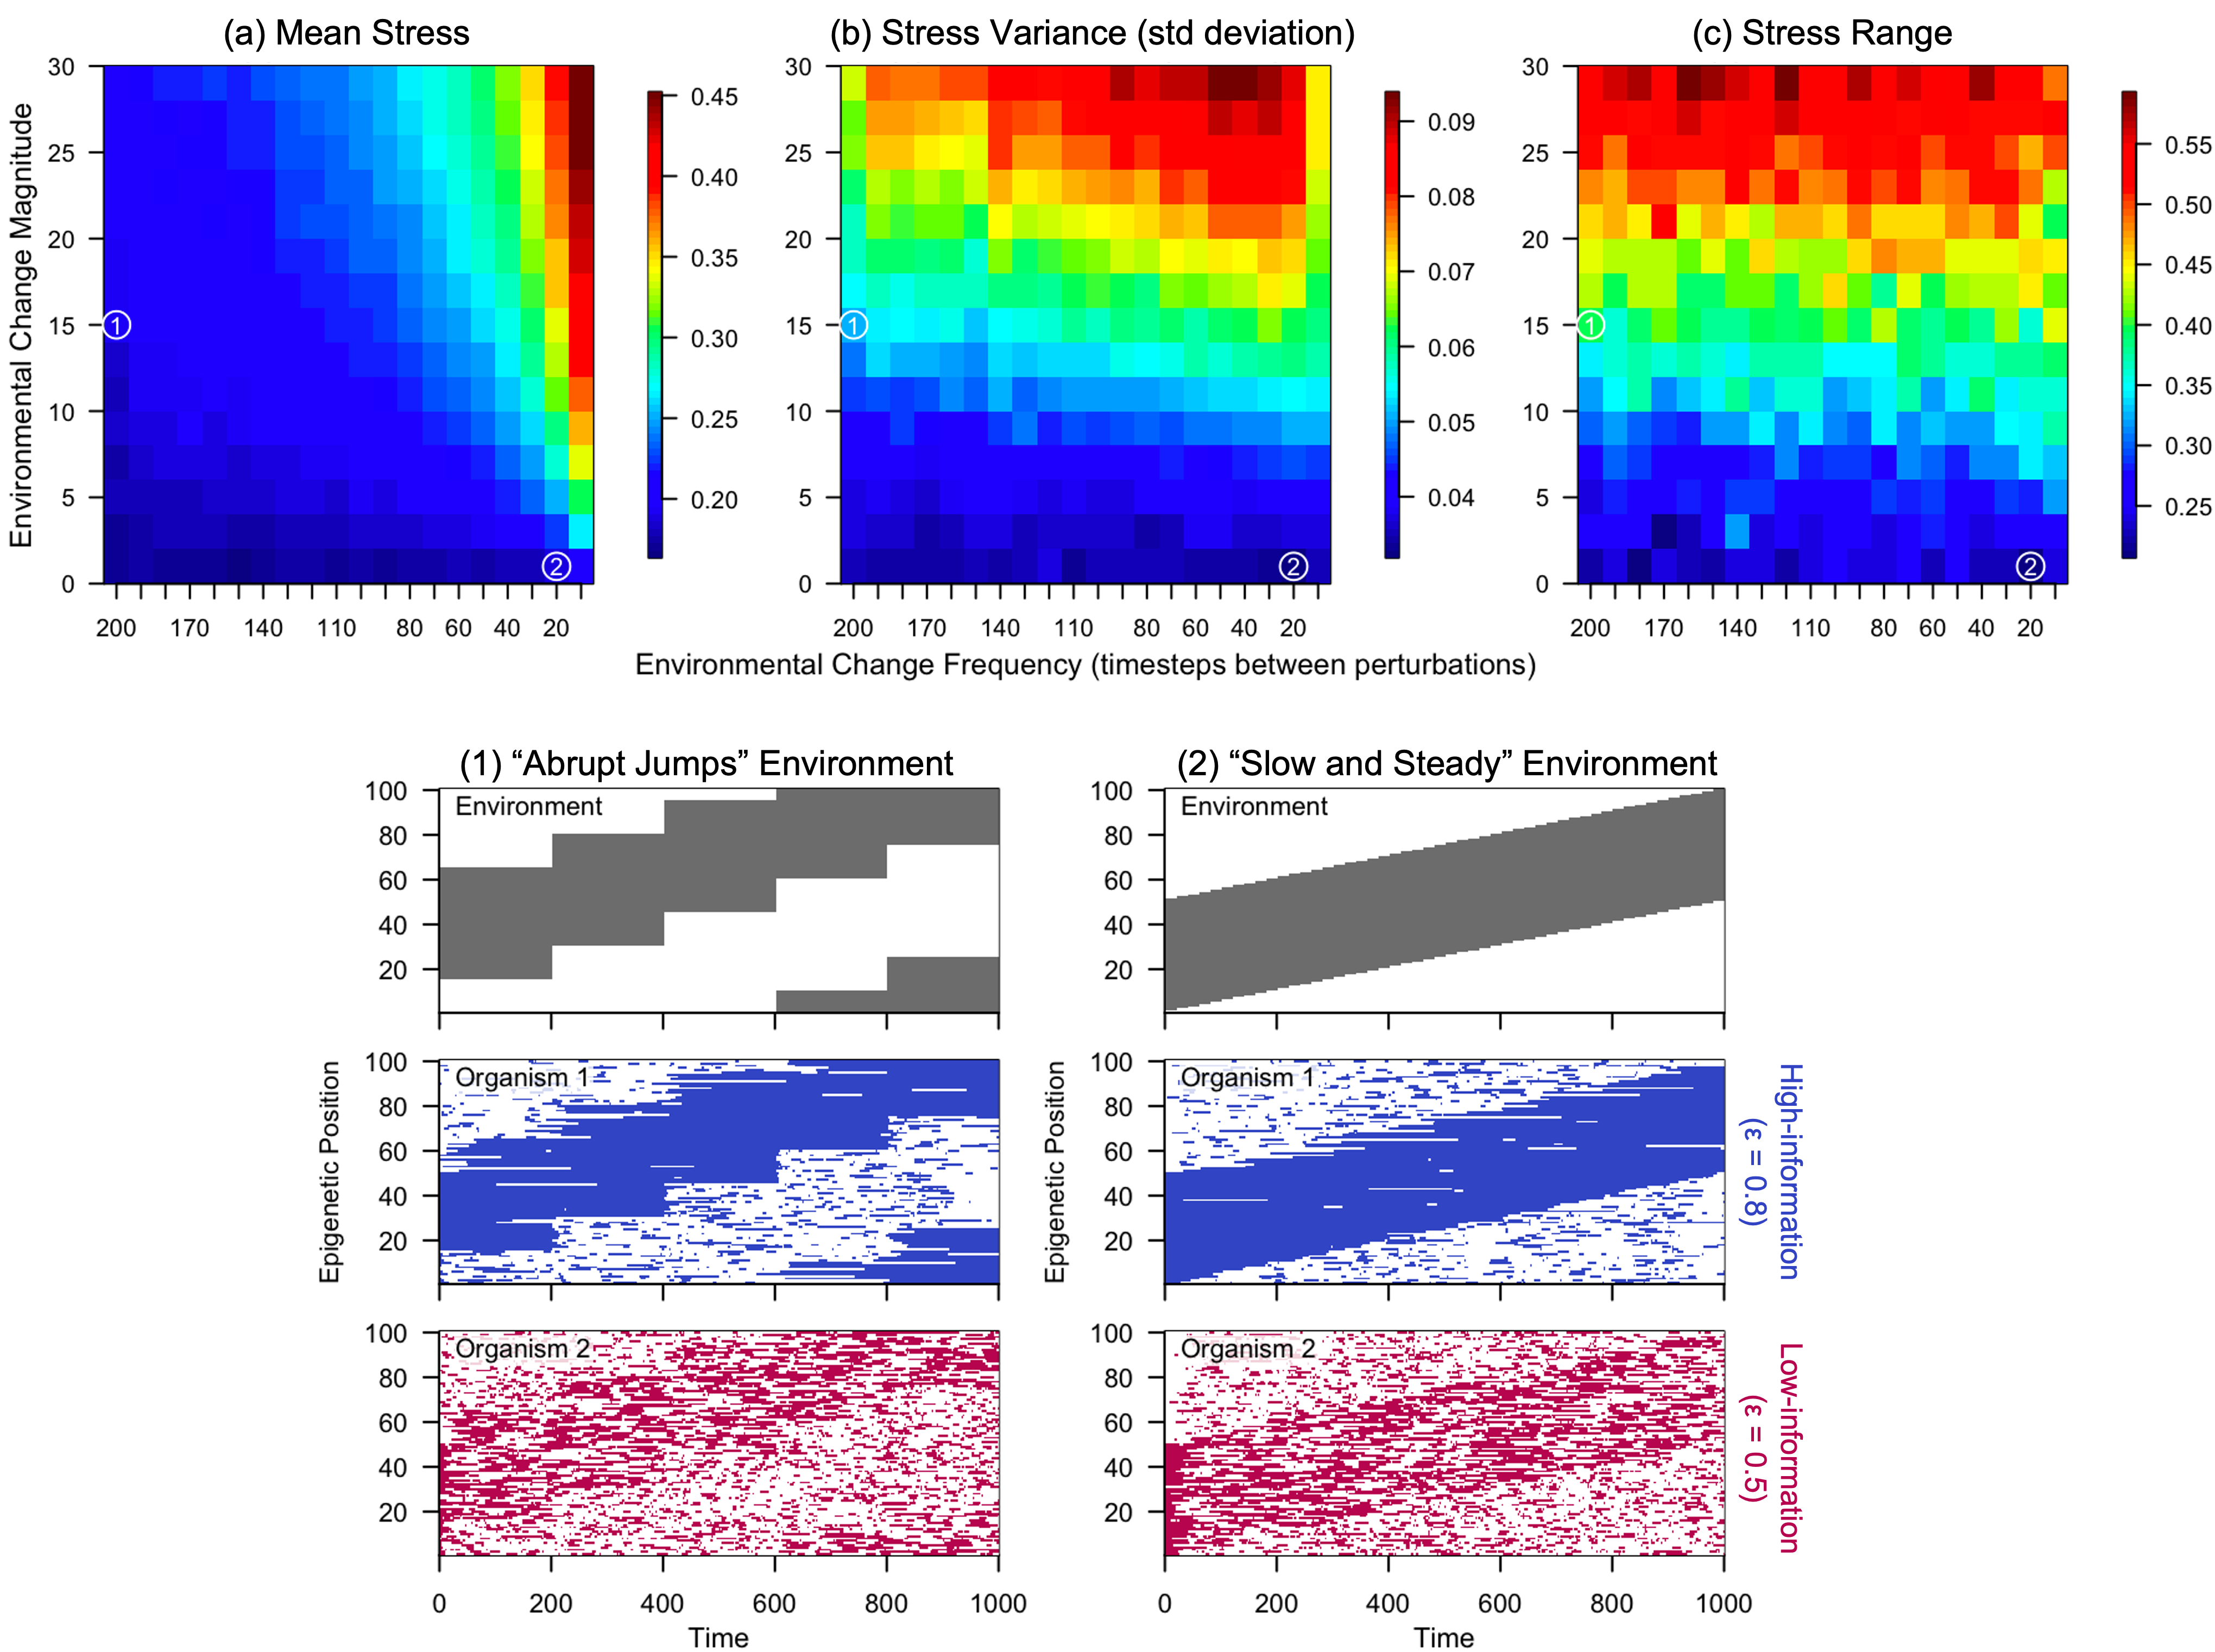
\includegraphics[width=\textwidth]{Figures/Fig_EnvironmentalSimulationComposite.png}
    \caption{\textbf{Effects of environmental change on organism performance.} (a) An organism with strong environmental tracking ($\epsilon = 0.99$) is able to track environments that change with low frequency or low magnitude. (b) However, high-magnitude changes result in large variance in stress levels, because of transient periods of re-equilibration to environmental conditions immediately following a shift in the environmental state. When changes are frequent and high-variance, stress variance actually decreases because of the extremely poor match to the environment. (c) Overall, larger magnitude shifts produce greater range in stress (comparing minimum to maximum values over the course of the simulation) because of periodic spikes in stress level. Below: Example scenarios (also marked on the heatmaps) for (1) low-frequency, intermediate-amplitude, and (2) high-frequency, low-amplitude environmental change. Filled area indicates a site with an epigenetic marker in the environment (top row, gray), an organism with a high degree of tracking (middle row, blue), and an organism with a low degree of tracking (bottom row, pink). Organisms with high levels of environmental information ($\epsilon = 0.99$) track better, especially in environments with larger magnitudes of change.}
    \label{fig:envirovar}
\end{figure}





% \clearpage

% \ 

% \clearpage

% \ 

% \clearpage

% \section{OLD TEXT/FIGURES:}

% \subsection{Coupling epigenetic rates}
% \textbf{This section will be deleted later.} One limitation of this model is that there is an ``obvious'' optimal solution: An organism that wishes to minimize its stress should simultaneously (1) minimize its probability of random demethylation (i.e., set $d_j = 0$), and (2) maximize its probability of preferential methylation (i.e., set $p_j$ very large). 

% This is in contrast to the ``original'' formulation of the model, in which stress drove epigenetic change in a fixed number of sites. (More stress = more sites changed.) In this case, if you ``ran out'' of sites to preferentially change, you would start changing non-preferred (i.e., incorrect) sites. So there was a ``natural coupling'' between tendencies for methylation and demethylation.

% There's some biology to think about here. Perhaps stress results in the production of enzymes that can catalyze epigenetic modification. These enzymes might be ``looking for something to do.'' Thus producing lots of these enzymes (having a high tendency) might result in more ``errors'' if all the preferential sites are already modified. This means that $d_j$ and $p_j$ might be coupled in some way.

% One way to do this is by assuming that $d_j$ and $p_j$ are related to one another, and to $m_j$, an individual's tendency for methylation.

% \subsubsection{OPTION 1: MEAN DEMETHYLATION IS PROPORTIONAL TO METHYLATION}

% We might assume that $d_j$ is some deviation $\epsilon$ less than $m_j$, and $p_j$ is the same deviation away in the opposite direction:

% \begin{equation}
%     m_j = \frac{\left( d_j - \epsilon \right) + \left( p_j + \epsilon \right)}{2}
% \end{equation}

% If we want the baseline rates of methylation and demethylation to differ, we can introduce the baseline multiplier $b$, which can take on values greater or less than 1 to represent greater or smaller tendencies to demethylate, respectively.

% \begin{equation}
%     m_j = \frac{b\left[ \left( d_j - \epsilon \right) + \left( p_j + \epsilon \right) \right]}{2}
% \end{equation}

% Similarly, we can treat $\epsilon$ as a proportional perturbation, e.g.:

% \begin{equation}
%     m_j = \frac{b\left[ d_j\left( 1 - \epsilon \right) + p_j \left( 1+ \epsilon \right) \right]}{2}
% \end{equation}
% Here, we choose $0 \leq \epsilon \leq 1$ so that all demethylation probabilities are nonnegative. \textbf{This is the version used in the current incarnation of the model.}

% \subsubsection{OPTION 2: PREFERENTIAL AND RANDOM DEMETHYLATION HAVE A FIXED COUPLING}

% We could also assume that $p_j$ and $d_j$ are related to one another in a fixed way. They could have a fixed difference, e.g.:
% \begin{equation}
%     p_j = d_j + \epsilon,
% \end{equation}
% or be proportional, e.g.:
% \begin{equation}
%     p_j = \epsilon d_j.
% \end{equation}

% \subsubsection{OTHER OPTIONS?}
% All suggestions accepted.

% \section{More on environmental tracking...}
% We demonstrated this phenomenon in our mathematical model by showing how different epigenetic tendencies intersected with the frequency of environmental change. 

% \textit{For now, I have a couple placeholder timeseries figures  (Figures \ref{fig:changerates}-\ref{fig:changerates2}), but I plan to make something more sophisticated in future.}

% \textit{One thing to think about here is that the higher your epigenetic tendencies are, the faster you're going to get to the stress minimum. Is there a natural ``upper bound'' on these tendencies? Like if you make them large, you have more variance in the population? Preliminary analyses (Figure \ref{fig:methyltendency}) didn't support this. Maybe if your rates are too fast, evolution doesn't work as well because there's more of a chance someone with a ``poor'' tendency just stochastically has the highest fitness?}

% \begin{figure}
%     \centering
%     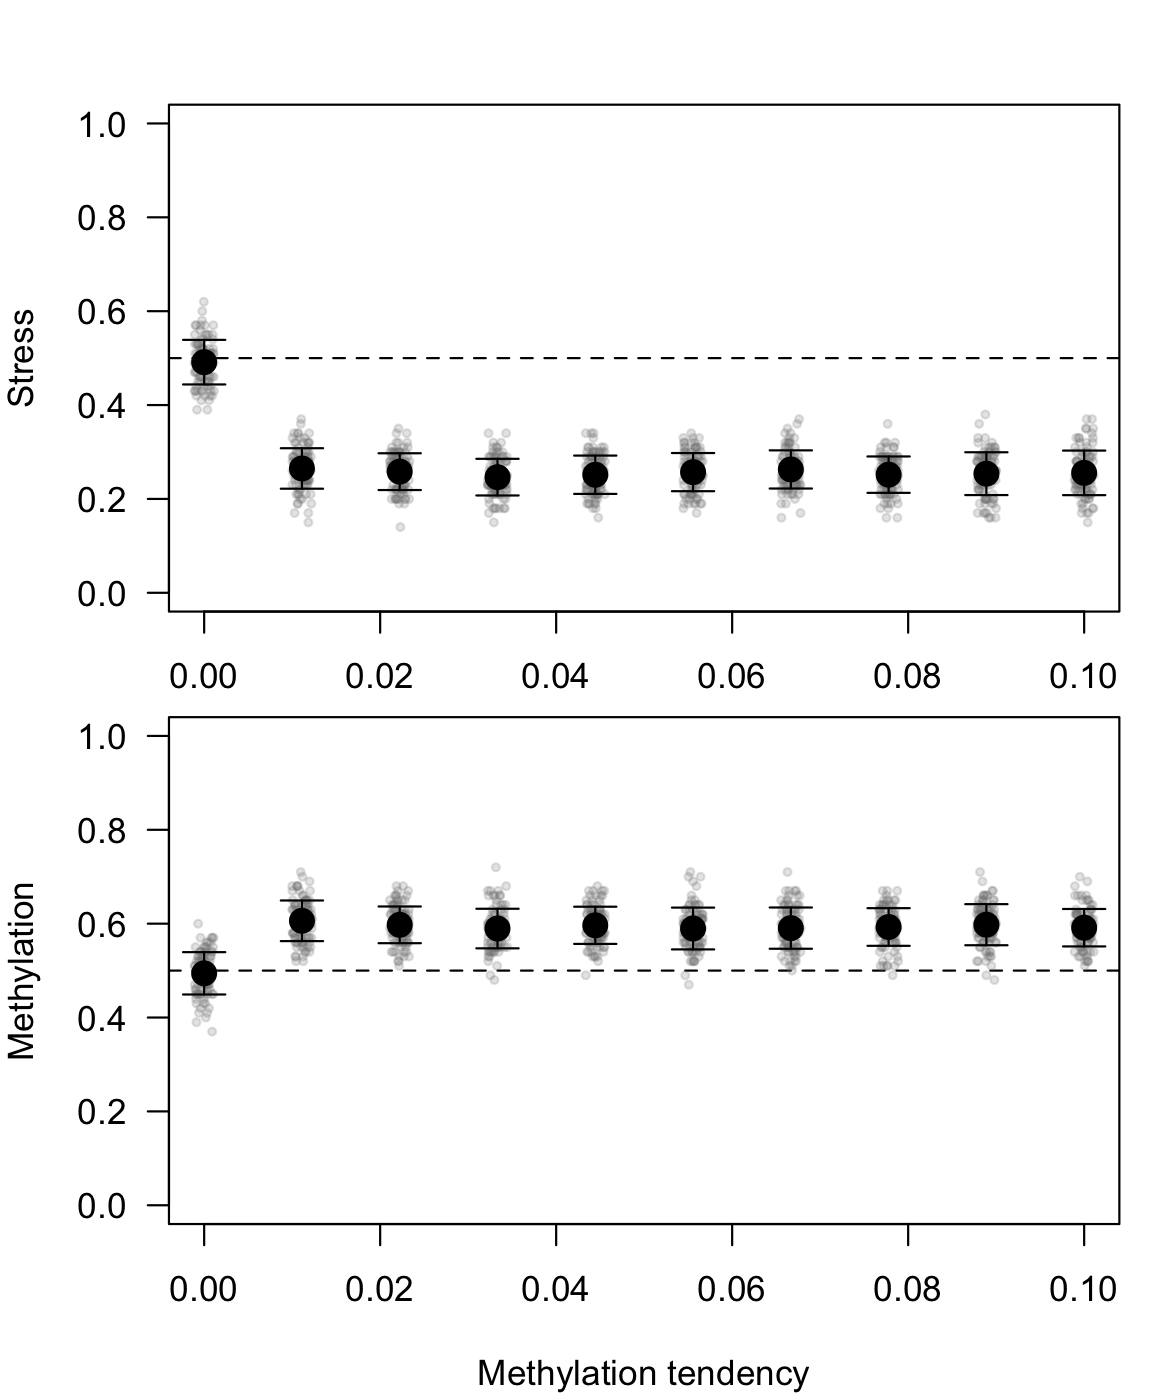
\includegraphics[width=0.8 \textwidth]{Figures/SFig_MethylationTendency.png}
%     \caption{Methylation tendency affects the rate of approach (not shown) but not the eventual stress levels or methylation rates that an organism experiences. Epsilon 0.8. Base multiplier 1. \textbf{This is for the supplement.}}
%     \label{fig:methyltendency}
% \end{figure}

% \begin{figure}
%     \centering
%     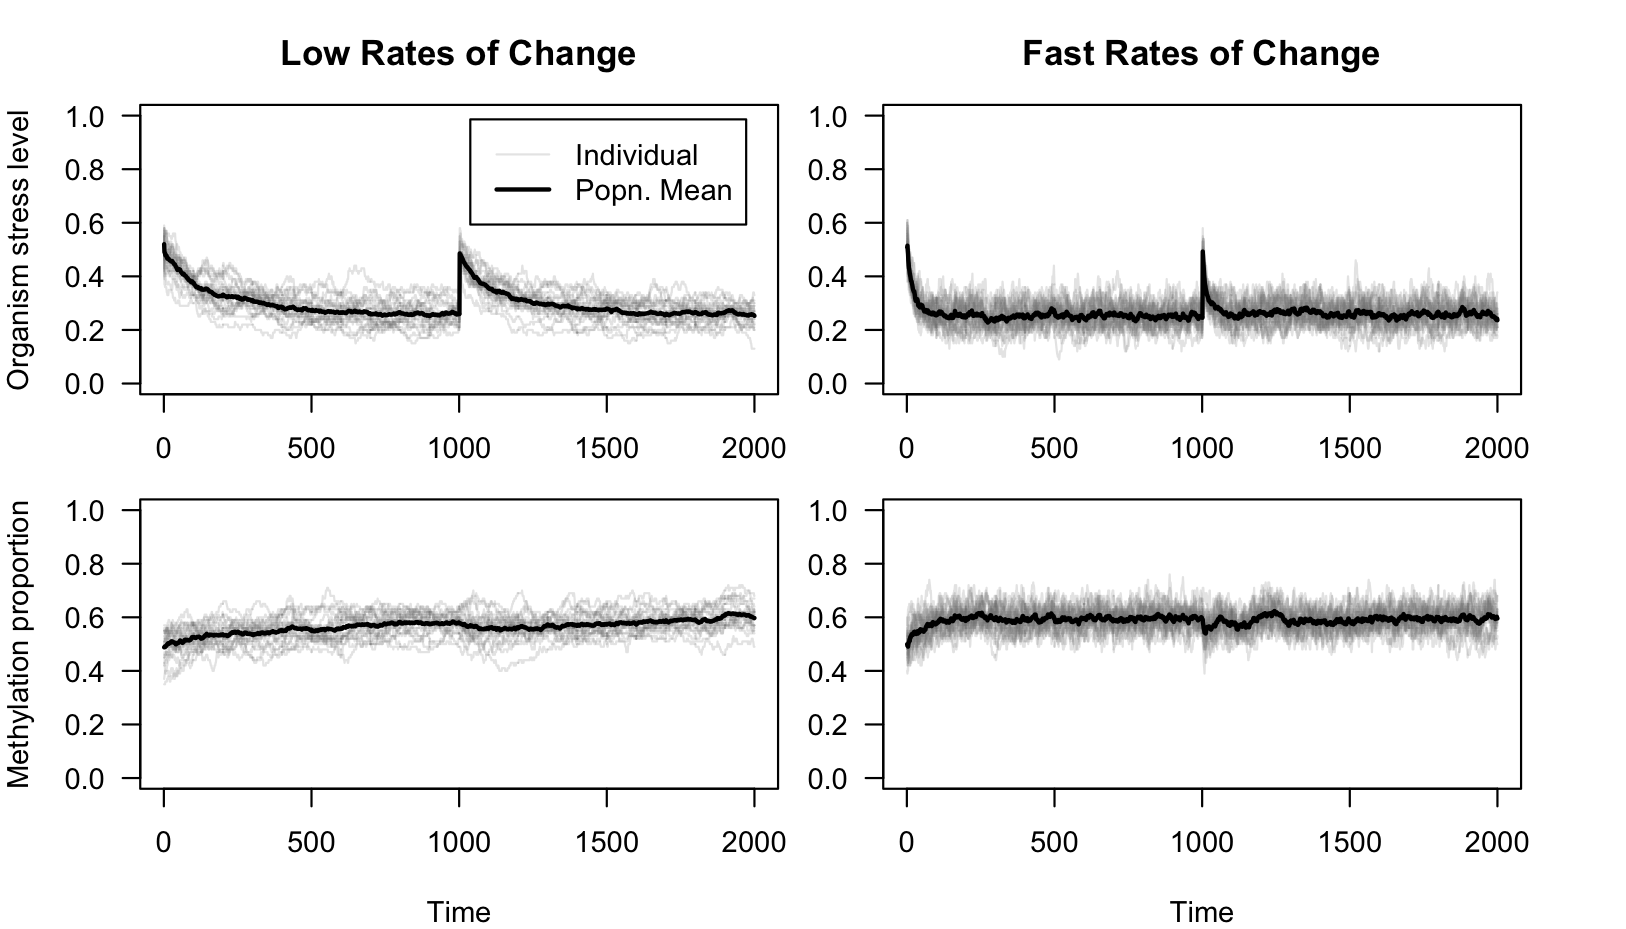
\includegraphics[width= 0.9 \textwidth]{Figures/Fig_ChangeRates.png}
%     \caption{Contrast in the time to minimum stress for two different epigenetic tendencies. Baseline methylation tendency of 0.01 (left; slow) and 0.1 (right; fast). Epsilon 0.8. Base multiplier 1.}
%     \label{fig:changerates}
% \end{figure}

% \begin{figure}
%     \centering
%     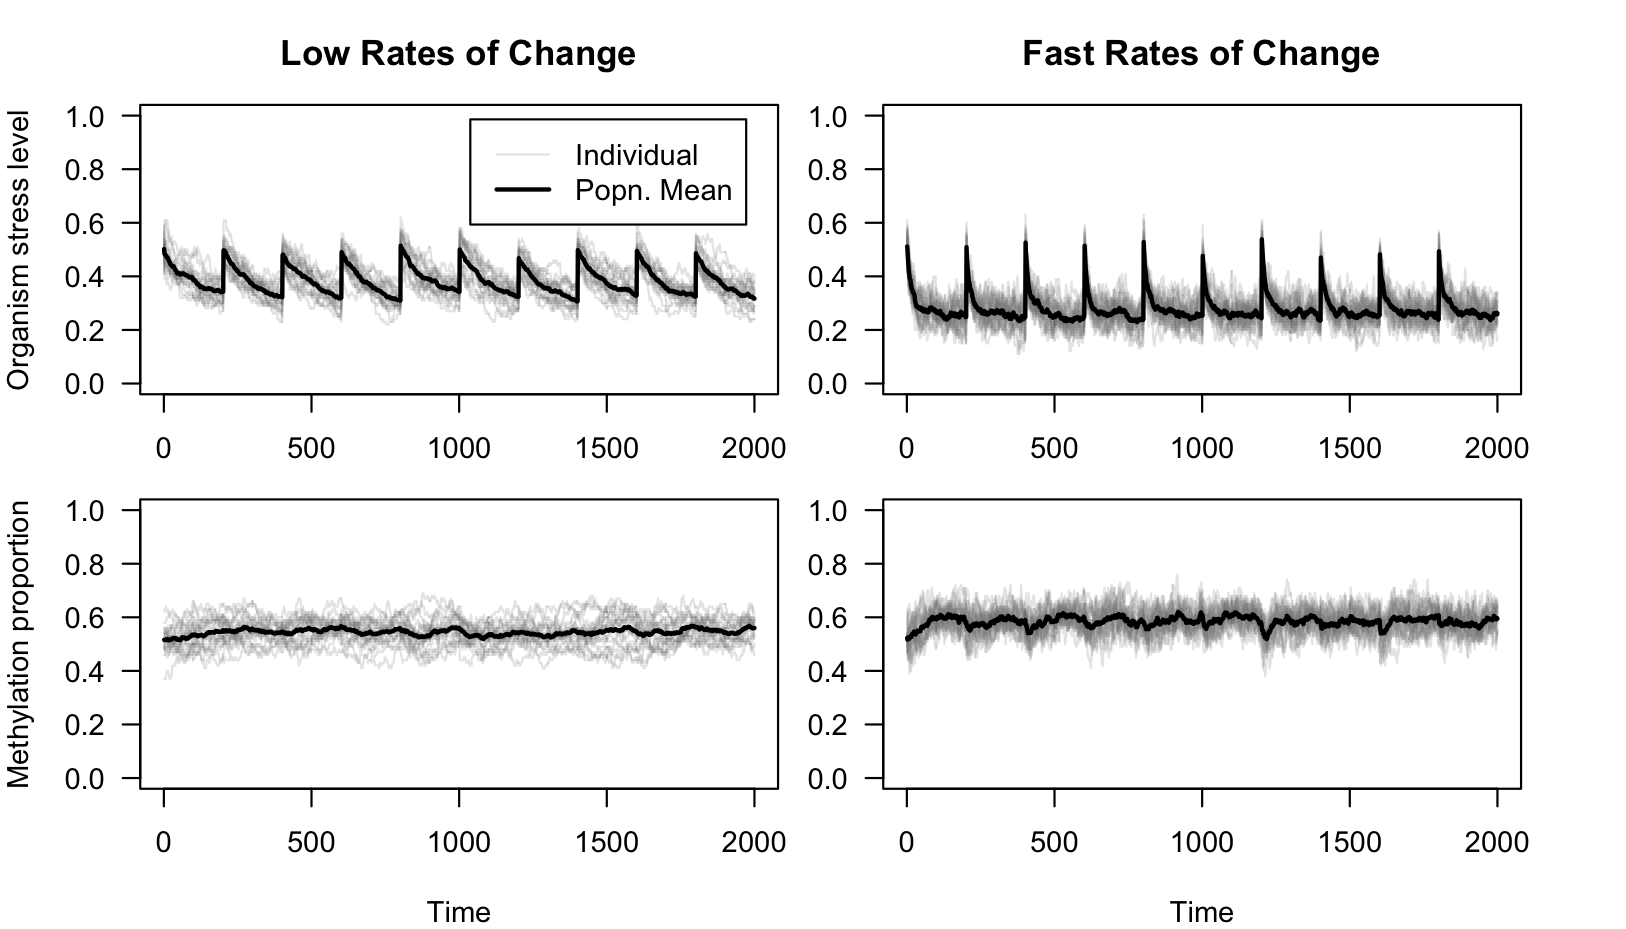
\includegraphics[width= 0.9 \textwidth]{Figures/Fig_ChangeRates_freqshifts.png}
%     \caption{Same organismal biology as Figure \ref{fig:changerates}, but with more frequent environmental change. Note that in this case, the organisms with relatively slow epigenetic change don't achieve low stress before the environment changes again. Baseline methylation tendency of 0.01 (left) and 0.1 (right). Epsilon 0.8. Base multiplier 1.}
%     \label{fig:changerates2}
% \end{figure}

% \subsubsection{Empirical Data}
% \subsubsection{Knowledge Gap}

\end{document}
